\documentclass[10pt]{beamer}

\usetheme[progressbar=frametitle]{metropolis}

\usepackage{booktabs}
\usepackage[scale=2]{ccicons}

\usepackage{pgfplots}
\usepgfplotslibrary{dateplot}

\renewcommand{\footnotesize}{\small}

\usepackage{xspace}
\newcommand{\themename}{\textbf{\textsc{metropolis}}\xspace}


\title{A Feasibility Study of \textsc{Concept Drift} in Empirical Software Engineering}
%\subtitle{\textsc{in Empirical Software Engineering}}
\date{\today} 
\author{Md Alamgir Kabir \\ Supervisor: Dr. Jacky Keung}

\institute{Department of Computer Science}
\titlegraphic{\hfill
\includegraphics[height=1.5cm]{cityu.png}}

\begin{document}

\maketitle

\begin{frame}{Topic}
  \setbeamertemplate{section in toc}[sections numbered]
  \tableofcontents[hideallsubsections]
\end{frame}

%%%%%%%%%%%%%%%%%%%%%%%%%%%%

\section{\textsc{Concept Drift}}

\begin{frame}{Concept Drift}
\begin{itemize}
  \item \textbf{Streaming data}: Incoming data of heterogeneous sources
  \item Behavior of these streaming data is changing over time
  \item \textsc{\textbf{Concept Drift  \footnote{Ditzler, G. (2015). Learning in Nonstationary Environments : A Survey, (November). \url{https://doi.org/10.1109/MCI.2015.2471196} } }:} The changes in the distribution or concept over time 
  \item A time changing probability distribution in high speed data streams
  \item Concepts are often not stable but change with time such as Weather Prediction and Customers’ Preference
\end{itemize}
\end{frame}

\begin{frame}{Concept Drift}
According to Lu \footnote{Lu, N., Zhang, G., \& Lu, J. (2014). Concept drift detection via competence models. Artificial Intelligence, 209(1), 11–28. \url{https://doi.org/10.1016/j.artint.2014.01.001}}, the problem can be framed as follows.
\begin{itemize}
    \item If we denote \textit{\textbf{the feature vector as x}} and the \textit{\textbf{class label as y}}, then the \textbf{\textit{data stream}} will be an infinite sequence of \textit{\textbf{(x, y)}}.
    \item If the concept drifts, it means the distribution of \textit{\textbf{p(x, y)}} is changing between the current data chunk
    \item If we decompose \textbf{\textit{p(x, y)}} into the following two parts as\textbf{ \textit{p(x, y) = p(x) × p(y|x)}}
    \item we could say there are two sources of concept drift: \textbf{\textit{one is p(x)}}, which evolves with time t, and can also be written as p(x|t)
    \item the \textbf{\textit{other is p(y|x)}}, the conditional probability of feature x
\end{itemize}
\end{frame}
%%%%%%%%%%%%%%%%%%%%%%%%%%%%
\section{Types of Concept Drift}
\begin{frame}{Types of Concept Drift}
According to Žliobaitė, \footnote{Žliobaitė, I. (2010). Learning under concept drift: an overview. arXiv preprint arXiv:1010.4784.}
\begin{figure}[ht]
  \begin{center}
  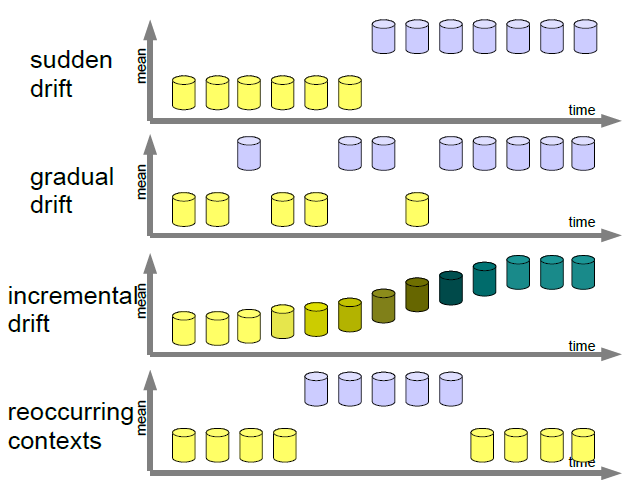
\includegraphics[width=8.3cm]{TypesofConceptDrift.png}
  \end{center}
  \caption{The four structural types of the drift}
  \label{tahapan_2}
\end{figure}
\end{frame}
%%%%%%%%%%%%%%%%%%%%%%%%%%%%
\section{Detecting Concept Drift}
\begin{frame}{Detecting Concept Drift}
The first attempt to handle of concept drift with case-based technique was IB3 (Instance-based) learning \footnote{Aha, D. W., Kibler, D., \& Albert, M. K. (1991). Instance-based learning algorithms. Machine learning, 6(1), 37-66.}.\\
Detecting concept drift-
\begin{itemize}
    \item Monitoring \textbf{raw data} (By data distribution)
    \item Monitoring \textbf{parameters of learners} (By parameters)
    \item Monitoring prediction \textbf{errors of learners} (By learners output)
\end{itemize}
\end{frame}

%%%%%%%%%%%%%%%%%%%%%%%%%%%%
\section{Practical Problem in Classification}
\begin{frame}{Practical problem in classification}
Being the environments non stationary it exhibits class imbalance that causes the practical problem in classification i.e., one of the most major problem in data mining and machine learning \footnote{Hoens, T. R., \& Chawla, N. V. (2012). Learning in non-stationary environments with class imbalance. In Proceedings of the 18th ACM SIGKDD international conference on Knowledge discovery and data mining - KDD ’12. \url{https://doi.org/10.1145/2339530.2339558}}.
\begin{itemize}
    \item It requires a lot of effort to observe the new minority class instances in new incoming data.
    \item The techniques of incremental learning in imbalance datasets (i.e., limited label data and plenty unlabeled data) with semi-supervised learning are more complex compare to the techniques of fixed distributions.
\end{itemize}
    
\end{frame}
%%%%%%%%%%%%%%%%%%%%%%%%%%%%
\section{Implications in Software Engineering Research}
\begin{frame}{Implications in SE Research/1}
\begin{itemize}
    \item Prediction model are developed by using historical datasets (i.e., fixed distributions) 
    \item Proposed models to predict the number and the location of future bugs in software source codes
    \item Such predictions can help the project manager to lead the project by proper utilizing the testing resources
    \item Unfortunately, the prediction model may not work if the historical datasets changes overtime \footnote{Ekanayake, J., Tappolet, J., Gall, H. C., \& Bernstein, A. (2009). Tracking concept drift of software projects using defect prediction quality. Proceedings of the 2009 6th IEEE International Working Conference on Mining Software Repositories, MSR 2009, 51–60.}
\end{itemize}
\end{frame}

\begin{frame}{Implications in SE Research/2}
\begin{itemize}
    \item Due to the change of some influencing features, bug generation process becomes more unsuitable. \footnote{Ekanayake, J., Tappolet, J., Gall, H. C., \& Bernstein, A. (2012). Time variance and defect prediction in software projects. Empirical Software Engineering, 17(4–5), 348–389.}
    \item They observed that the change in number of author editing a file and a number of defects fixed by them introduce the concept drift.
    \item They have also seen that the prediction quality significantly varies over time. 
\end{itemize}
\end{frame}

\begin{frame}{Implications in SE Research/3}
\begin{figure}[ht]
  \begin{center}
  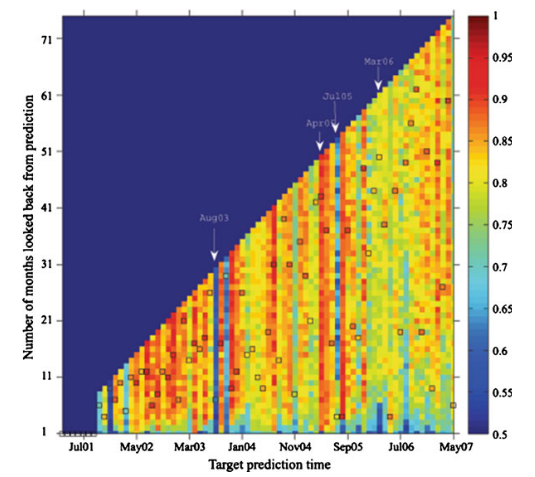
\includegraphics[width=7cm]{TargetPredictionTime.PNG}
  \end{center}
  \caption{Eclipse heat-map: Prediction quality using different training periods with the points of highest AUC highlighted} 
  \label{tahapan_3}
\end{figure}
\end{frame}

\begin{frame}{Implications in SE Research/4}
\begin{itemize}
    \item The maximum \textbf{AUC values} for each target period typically lie on neither ends.
    \item \textbf{The models should not be trained on data collected from a very long or very short history.} \footnote{Ekanayake, J., Tappolet, J., Gall, H. C., \& Bernstein, A. (2012). Time variance and defect prediction in software projects. Empirical Software Engineering, 17(4–5), 348–389.}
\end{itemize}
\end{frame}


%%%%%%%%%%%%%%%%%%%%%%%%%%%%

\begin{frame}{Current studies demand...}
\begin{itemize}
        \item Current studies demand to do the several experiments in the area of empirical software engineering to prepare the \textbf{\textit{well trained prediction model in streaming datasets}}.
        \item We have planned a set of experiments in the datasets of \textbf{\textit{open source projects}}. 
\end{itemize}

\end{frame}



\plain{Thank you so much for listening!}

%\begin{frame}[allowframebreaks]{References}

%  \bibliography{demo}
%  \bibliographystyle{abbrv}

%\end{frame}

\end{document}


